% !TEX program = lualatex
% Overleaf でコンパイル時は Menu -> Compiler を "LuaLaTeX" に設定してください
% (XeLaTeX でも動くように xeCJK を併記したい場合は documentclass を切り替えてください)

\documentclass[11pt,a4paper]{ltjsarticle}

\usepackage{luatexja-fontspec}
\usepackage{geometry}
\geometry{margin=22mm}

\usepackage{graphicx}
\usepackage{booktabs}
\usepackage{array}
\usepackage{caption}
\usepackage{subcaption}
\usepackage{xcolor}
\usepackage{hyperref}
\hypersetup{colorlinks=true, linkcolor=blue!60!black, citecolor=blue!60!black, urlcolor=blue!60!black}
\usepackage{enumitem}
\setlist{itemsep=2pt, topsep=2pt}

\usepackage{amsmath}
\usepackage{amssymb}
\usepackage{fancyhdr}
\pagestyle{fancy}
\fancyhf{}
\fancyhead[L]{FlyWire connectome: 側抑制の連結体解析}
\fancyhead[R]{\thepage}

\title{ショウジョウバエ視覚系における側抑制の連結体解析\\
\large -- FlyWire データセットを用いた量的検証}
\author{Keisuke Toyoda}
\date{\today}

\begin{document}
\maketitle

\begin{abstract}
ショウジョウバエ視覚系では「至るところで側抑制 (lateral inhibition) が起きている」と古典的に言われる。本報告では、FlyWire の全脳連結体データ (約 14 万ニューロン / 910 万エッジ) を用いて、この主張を 9 つの問いに分解して定量検証した。主要な結果として
(1) 視覚系の全シナプスの約 44\% が抑制性で、抑制 dominant cell type は少数派ではなく cell type レベルで多数派である、
(2) Δcolumn 単位の lateral spread を計算した結果、抑制 dominant cell type は興奮 dominant の約 3.35 倍広いカラム範囲をカバーする、
(3) Lamina amacrine (Lai)、Medulla の Pm/Dm 系、UV color circuit の Dm8 などの古典的側抑制回路が連結体レベルで再現される、
(4) medulla 境界部の cell では入力シナプス数が中央部の 30–75\% に減るが、E/I balance はほぼ保たれるという「scale down but preserve ratio」型の構造を持つ、
(5) この境界効果は projection 型のニューロン (T4/T5) で相対的に弱く、columnar 受け手 (L1--L5, Mi 系) で強い、
ことを示す。さらに、配線構造から計算を推定する拡張解析 (Q10--Q13) として、(6) ON/OFF 運動検出器 T4/T5 の方向選択性が興奮・抑制入力の\textbf{空間オフセット}として連結体に刻まれていること (亜型 a/b/c/d で入力 dipole 軸が回転し、対向ペアは反平行・水平/垂直ペアは直交、両半球で一致)、(7) columnar 標的は中心興奮・(二シナプス性) 周辺抑制からなる\textbf{Mexican-hat 受容野}を持ち空間バンドパス特性を予測できること、(8) 全抑制シナプスの約 41\% が抑制性細胞を標的とする\textbf{脱抑制}であること、(9) 抑制が M 層ごとに役割分担すること (Dm 遠位・Pm 近位) を示した。連結体解析は紙上の解剖記述を量的に裏付ける一方で、ML 推定の神経伝達物質ラベルの誤りや、機能補償が連結体外 (gain control 等) で行われている可能性など、いくつかの限界も明らかになった。
\end{abstract}

\section{はじめに}\label{sec:intro}

ショウジョウバエ視覚系 (lamina, medulla, lobula, lobula plate からなる視葉) は、約 800 個眼の retinotopic な hex 格子状処理が中央計算 (中心脳) へと収束する典型的なパラレル並列計算系である。古典的な解剖・電気生理学的研究は、ラミナの Lai (lamina amacrine)、medulla 中央〜深層の Dm/Pm 系 (distal/proximal medulla intrinsic)、Dm8 (UV color processing)、全 medulla を 1 個でカバーする CT1 など、多数の抑制性インターニューロンが各層で「側抑制 (lateral inhibition)」を提供することを記述してきた。

しかし、これらの記述は個別細胞型に対する個別観察の積み重ねで、視覚系全体としてどれくらいの規模の抑制配線があり、空間的にどのスケールで広がっているかを連結体レベルで横断的に量化したものは少ない。本報告では、FlyWire の全脳連結体データ \cite{flywire2024} を用いて、視覚系の側抑制を 9 つの問い (Q1--Q9) に分解して定量解析した結果をまとめる。

\subsection*{問いの一覧 (Q1--Q13)}

\begin{description}[leftmargin=2em, style=nextline]
\item[Q1] 視覚系の全シナプスのうち、抑制性 (GABA / GLUT / HIS) はどれくらいの割合か?
\item[Q2] 抑制性出力をメインに持つ cell type はどれくらい広範に存在するか?
\item[Q3] 同タイプ間 (within-type) の抑制接続はどの程度起きているか?
\item[Q4] wide-field な抑制 (1 ニューロンの出力シナプスが広い column 範囲に分布) は本当に抑制 dominant cell type で顕著か?
\item[Q5] 既知の側抑制回路 (Lai, Dm/Pm 系) が連結体データで再現されるか?
\item[Q6] Dm8 (UV color circuit) のような cell では、出力先が columnar でないため Q4 metric が適用できない。input-side で receptive field を測れるか?
\item[Q7] 端 column の cell は隣接 column が少ないので、本来側抑制を片側からしか受けられないはず。何らかの補償機構があるか?
\item[Q8] 抑制性インターニューロン全体を family 単位で網羅サーベイすると何が見えるか?
\item[Q9] Q7 の端効果パターンは columnar 受け手 cell type 全般で成立するか? それとも一部に例外があるか?
\item[Q10] T4/T5 の方向選択性は、興奮・抑制入力の空間配置 (オフセット) として連結体に現れるか?
\item[Q11] columnar 標的は中心興奮・周辺抑制 (center--surround) の受容野を connectome から再構成できるか?
\item[Q12] 抑制の回路トポロジー (feedforward / feedback / 相互抑制 / 脱抑制) はどうなっているか?
\item[Q13] 抑制は medulla の M 層 (深さ) でどう役割分担しているか?
\end{description}

Q1--Q9 が側抑制の「量・空間スケール」を量化するのに対し、Q10--Q13 は\textbf{配線構造から計算を推定する}拡張である (\S\ref{sec:extended})。

\section{データと手法}\label{sec:methods}

\subsection{データセット}

FlyWire (\href{https://flywire.ai}{flywire.ai}) の v783 公開連結体データを用いる。本解析では特に以下の CSV を利用する。
\begin{itemize}
\item \texttt{neurons.csv} (139{,}256 行): 各ニューロンの \texttt{root\_id}, neurotransmitter type (\texttt{nt\_type}) の機械学習推定値, 信頼度スコア
\item \texttt{classification.csv} (139{,}256 行): cell class / sub\_class / hemisphere
\item \texttt{consolidated\_cell\_types.csv}: 各 \texttt{root\_id} の primary cell type (Mi1, T4a, Dm9 等)
\item \texttt{connections\_princeton\_no\_threshold.csv}: シナプス接続テーブル (pre/post root\_id, syn\_count, neuropil, nt\_type)
\item \texttt{column\_assignment.csv} (45{,}061 行): hex 格子上の medulla 個眼柱への割り当て (\texttt{(p, q)} hex coords + hemisphere, 31 種の columnar cell type が対象)
\item \texttt{synapse\_coordinates.csv} (34{,}156{,}320 行): 個々のシナプスの 3D 物理座標
\end{itemize}

\subsection{解析パイプライン}

データロードは \texttt{src/data/FlyWireDataManager} で行い、Optic Lobe (lamina + medulla + lobula + lobula plate) に属する 90{,}810 個のニューロンと、それらの間の 9{,}100{,}647 個のエッジに絞って解析した。

\subsubsection*{抑制性 / 興奮性の分類}

Drosophila では GABA (GABA-A 受容体経由)、HIS (HCl1 受容体)、GLUT (GluCl 受容体経由でしばしば抑制性) を抑制性とみなし、ACH を興奮性とした。\texttt{nt\_type} の多くは機械学習推定値であり、R1-6 photoreceptor のみドメイン知識から HIS にハード補正してある。

\subsubsection*{Δcolumn metric}

\texttt{column\_assignment.csv} の \texttt{(p, q)} を axial hex coords とみなし、cell 間の hex 距離を以下で計算する。

\begin{equation}
d_\text{hex}(\Delta p, \Delta q) = \frac{|\Delta p| + |\Delta p + \Delta q| + |\Delta q|}{2}
\end{equation}

各 cell の出力シナプスを post の \texttt{(p, q)} で集計し、syn\_count で重み付けた centroid からの hex 距離の weighted mean を「lateral spread (column 単位)」と定義する。抑制 / 興奮 dominant の分類は、Q2 と同じく各 cell type の全出力 synapse 数を sign ごとに集計した synapse-weighted 分類を用いる。

\subsubsection*{Mi1 を proxy とする column 投影}

Tm5*/Sm 系などの wide-field 細胞は \texttt{column\_assignment.csv} に含まれないため、これらを post とするシナプスは直接 column 化できない。そこで、Mi1 (1-per-column かつ medulla-intrinsic) の物理 centroid と \texttt{(p, q)} の対応関係 (Spearman $\rho \approx 0.94$ で検証済み \cite{column_validation}) を利用し、各シナプスの最も近い Mi1 を \texttt{scipy.spatial.cKDTree} で求めて、その Mi1 の column を「そのシナプスの column」とする近似投影を行った。

\subsubsection*{拡張解析 (Q10--Q13) の手法}

\textbf{入力 dipole と円形統計 (Q10).} 各標的 cell について、columnar な入力源の \texttt{(p, q)} を \texttt{syn\_count} で重み付けた重心を home column 基準の $(\Delta p, \Delta q)$ で求め、cartesian 変換後に per-cell の dipole ベクトル (T4: $\mathrm{Mi9}-\mathrm{Mi4}$、T5: $\mathrm{Tm9}-\mathrm{Tm2}$) を構成する。亜型ごとにその角度の円形平均・resultant $R$・Rayleigh 検定 (非一様性) を計算する。端 column の入力非対称を避けるため hex 近傍が 5 個以上の内部 cell に限る。

\textbf{二シナプス性 surround (Q11).} 抑制 partner $J \to T$ について、$J$ の columnar 興奮入力の column を $T$ の home 基準で集計する (重み = $J\to T$ シナプス数 $\times$ $J$ の各入力 column の重み)。これを $\Delta$ ごとに足し上げ、抑制が「見ている」視空間 (surround) を再構成する。

\textbf{M 層深さ (Q13).} 右半球 Mi1 の synapse 重心群を PCA した最小分散軸を局所深さ法線とし、Mi1 の深さ分布の 1--99\%tile を medulla 厚 $[0, 1]$ に較正する。多神経網細胞 (CT1 や Tm9 の lobula arbor 等) は medulla 窓 $[-0.25, 1.25]$ でクリップする。

\section{結果}\label{sec:results}

\subsection{Q1: 全シナプスの I/E バランス}\label{sec:q1}

視覚系全 9{,}100{,}647 エッジ (合計 32{,}851{,}872 シナプス) を \texttt{nt\_type} で分類した結果、抑制性 (GABA + GLUT + HIS) は 14{,}351{,}911 シナプス (43.7\%)、興奮性 (ACH) は 18{,}359{,}592 (55.9\%)、その他 (DA/SER/OCT) は 140{,}369 (0.4\%) であった (図 \ref{fig:nt_dist})。
$I / (I + E) = 43.9\%$ で、視覚系の入力配線の半分近くを抑制が占めるという結果は「至るところで抑制がある」という主張と強く整合する。

\begin{figure}[htb]
\centering

\includegraphics[width=0.85\textwidth]{figures/fig1_nt_distribution.png}
\caption{視覚系全エッジを神経伝達物質タイプ別に集計したシナプス数。赤 = 興奮性 (ACH)、青 = 抑制性 (GABA, GLUT, HIS)、灰色 = モジュレータ / 不明 (DA, SER, OCT, NaN)。}
\label{fig:nt_dist}
\end{figure}

\subsection{Q2: 抑制性出力 dominant な cell type の広がり}\label{sec:q2}

>=1000 outgoing synapses を持つ主要 cell type は 344 種類存在し、そのうち $\text{inh\_frac} \geq 0.5$ (= 抑制性出力 dominant) なものは 206 種類 (60\%)、$\text{inh\_frac} \geq 0.95$ (= ほぼ純粋に抑制性) なものは 196 種類 (57\%) であった (図 \ref{fig:inh_frac_dist})。

\begin{figure}[htb]
\centering

\includegraphics[width=0.7\textwidth]{figures/fig2_inh_fraction_dist.png}
\caption{主要 344 cell types を $\text{inh\_frac}$ (= inh / total syn) の値で histogram にしたもの。0 近傍 (純興奮) と 1 近傍 (純抑制) に bimodal なピークが立ち、中間的 (mixed) な type は少ない。抑制 dominant type が大半を占める。}
\label{fig:inh_frac_dist}
\end{figure}

抑制ニューロンは少数の専門集団ではなく、連結体の cell type 多数派と言ってよい構成である。

\subsection{Q3: within-type の自タイプ抑制}\label{sec:q3}

「同じ primary\_type のニューロン同士で抑制し合う」のは最も直接的な側抑制 (同じ機能ユニットの隣同士で抑え合う) のシグナルである。inh / exc 両方を $\geq 500$ syn 持つ 58 type のうち、抑制側の自タイプ targeting 率が興奮側より高いのは 24 種 (41\%) であった。half 未満であることから、within-type lateral inhibition は支配的な機構ではなく、\textbf{側抑制の多くは専用の抑制 interneuron (Lai, Dm, Pm 系) 経由で起きている}ことが示唆される (Q4, Q5 で確認)。

\subsection{Q4: Δcolumn 単位の lateral spread}\label{sec:q4}

各 pre cell について、columnar target (\texttt{column\_assignment.csv} 入り)の (p,q) を syn\_count で重み付けた centroid を求め、各 target からの hex 距離の weighted mean を「column 単位の lateral spread」とした (図 \ref{fig:spread_dist}, \ref{fig:hex_footprint})。Q4 で直接観測できる同半球 columnar target は全 optic-lobe synapse の 35.2\% であり、この metric は全出力の部分観測である。

\begin{figure}[htb]
\centering

\includegraphics[width=\textwidth]{figures/fig3_column_spread_inh_vs_exc.png}
\caption{抑制 dominant (n=66) と興奮 dominant (n=24) cell type の lateral spread 分布の比較。左: weighted-mean Δcolumn の分布。右: 出力先 column 数の分布。抑制 dominant は spread 中央値 3.29、column 数中央値 69 で、興奮 dominant の 0.98 / 12 に対しそれぞれ約 3.35 倍 / 5.73 倍大きい。}
\label{fig:spread_dist}
\end{figure}

\begin{figure}[htb]
\centering

\includegraphics[width=\textwidth]{figures/fig4_hex_footprint.png}
\caption{代表的な cell の hex 格子上の出力 footprint。Pm08, Pm04, Dm4, Dm12 のような wide-field 抑制 interneuron は数十柱に及ぶ広いパッチを作るのに対し、Lai は中規模 (lamina 内)、Mi1 は ほぼ 1 柱に集中。$\times$ は weighted centroid、灰色は同半球の全 column 背景。}
\label{fig:hex_footprint}
\end{figure}

具体的な数値: Pm08 = 73 columns (spread 2.97), Pm04 = 62 (2.86), Dm4 = 23 (1.87), Dm12 = 30 (1.63), Lai = 9 (1.60), Mi1 = 12 (0.74), Tm9 = 11 (1.01), L2 = 7 (0.24)。\textbf{抑制 dominant cell type は興奮 dominant の約 3.35 倍 lateral に広がる}という、教科書通りの wide-field inhibition が連結体レベルで明確に検出された。

\subsection{Q5: 古典回路の検証}\label{sec:q5}

\paragraph{Lamina amacrine (Lai).}
古典的にラミナの L1/L2/L3 と R1-6 を、隣の個眼柱由来の信号で抑える GABA 性インターニューロン。本データで Lai の出力は 99\% が lamina (LA\_R/LA\_L) に位置し、ターゲットは L1/L2/L3/R1-6/Lai を含む (古典回路を再現)。シナプス数で重み付けすると GABA 30,505 > ACH 28,874 で僅かに GABA dominant。エッジ数ベースだと ACH と GABA がほぼ半々で、Lai 個体ごとの ML nt\_type 予測にバラツキがある。

\paragraph{Medulla の Dm / Pm 系.}
Dm 24 種 / Pm 14 種のうち多数が GABA / GLUT dominant で、medulla の Mi/Tm 系を広く支配する。教科書的な wide-field inhibition と整合 (Dm4, Dm12, Dm3p, Pm 全種など)。\textbf{ただし Dm9 は例外}: 文献では GABA 性とされるが FlyWire の ML 予測では出力の 97\% が ACH (syn 数ベース)。Dm9 の出力 spread (1.13) は他の Dm と同程度の wide-field なので形態は Dm 系に矛盾しない — つまり ML の nt\_type 予測の誤りか、Dm9 ラベルに別細胞が混入している可能性が高い。

\subsection{Q6: Dm8 (UV color circuit) の input-side metric}\label{sec:q6}

Dm8 (本データでは Dm8a 367 cells / Dm8b 406 cells に細分化) は medulla intrinsic な wide-field interneuron で、UV photoreceptor (R7) の入力を統合する古典的な color circuit 細胞。出力先 (Tm5a/b/c/d, Sm 系, Dm9 等) はすべて \texttt{column\_assignment.csv} に含まれないため、Q4 metric では評価できない。
代わりに、R7 (column\_assignment 内, 922 cells) を input として各 Dm8 cell が何個の unique R7 column から入力を受けるかを集計した (図 \ref{fig:dm8_input})。

\begin{figure}[htb]
\centering
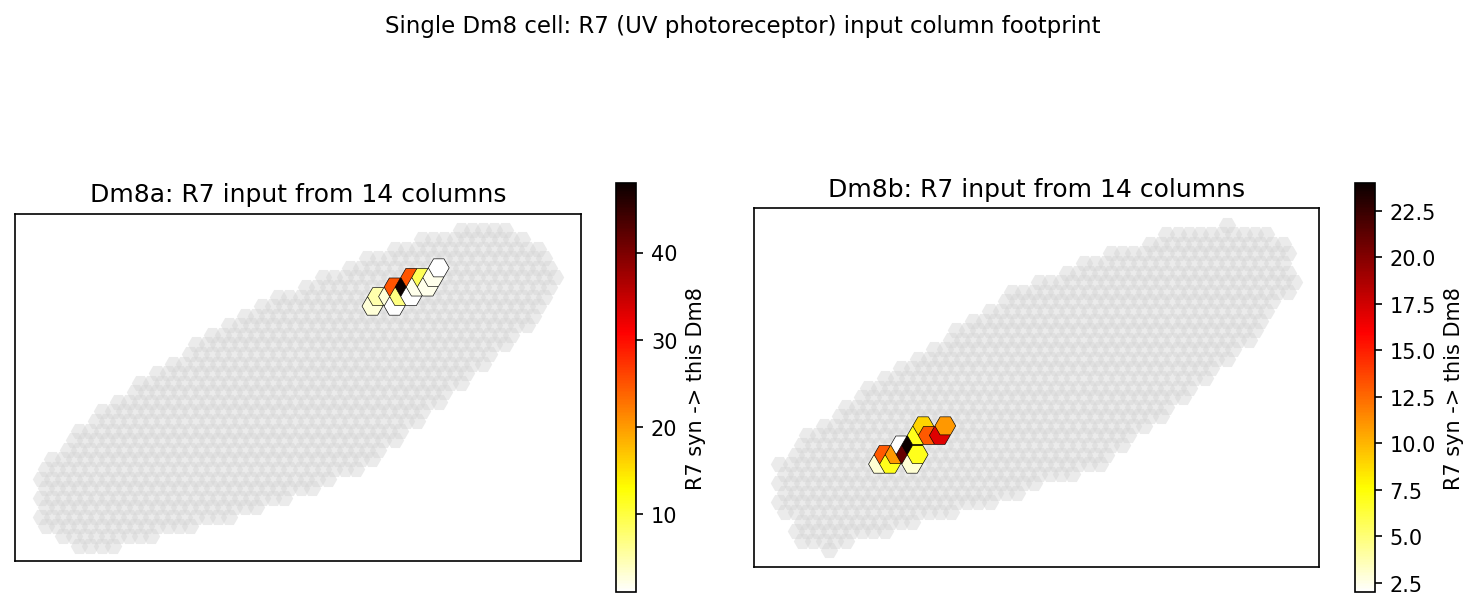
\includegraphics[width=0.85\textwidth]{figures/fig5_dm8_input_footprint.png}
\caption{Dm8a と Dm8b の代表 cell (R7 入力 column 数最大の cell) の R7 input column footprint。教科書記述の「home column + 周辺 14 個眼の R7 を集積」と一致する wide-field receptive field を hex 格子上に確認できる。}
\label{fig:dm8_input}
\end{figure}

集計結果: Dm8a (n=367)、Dm8b (n=406) ともに median 7 unique R7 input columns (range 1--14)。教科書記述 (Gao et al. 2008 \cite{gao2008}, Karuppudurai et al. 2014 \cite{karuppudurai2014}) の「home column + $\sim$14 周辺個眼の R7 入力を集積」と完全に一致。

\subsubsection*{Dm8 の input vs output column footprint}

Mi1 を nearest-neighbor proxy として Dm8 出力を column 空間に投影した結果、Dm8a で median 5 output columns (out/in 比 0.71)、Dm8b で median 4 (0.67)。\textbf{Dm8 は wide-field input integration ($\sim$7 columns) + 局所 output ($\sim$4--5 columns at home column)} という「wide input + narrow output」の構造を持つ。これは古典的な Dm8 home column architecture と整合する (Pm08 のような「広く撒く」wide-field 抑制とは別タイプの lateral interneuron)。

\subsection{Q7: 端 column の Mi1 と中央 column の比較}\label{sec:q7}

medulla の hex 格子の端にある column は隣接 column が少ない (3-5 個) ので、側抑制が「隣接 column から来る」のなら端 column では本来抑制が不足するはずである。何らかの補償機構があるかを Mi1 (1-per-column な columnar 受け手) で調べた (図 \ref{fig:edge_mi1})。

\begin{figure}[htb]
\centering
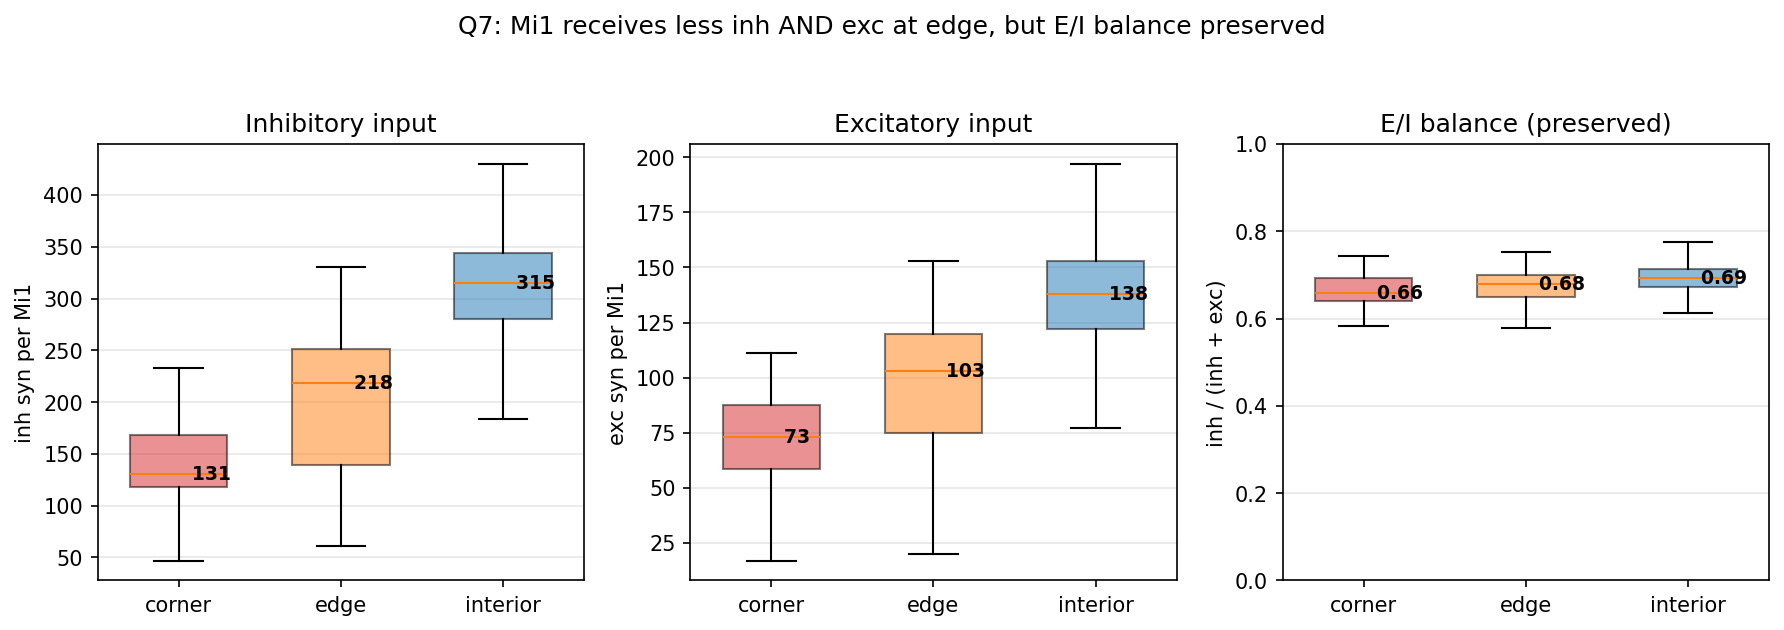
\includegraphics[width=\textwidth]{figures/fig6_edge_effect_mi1.png}
\caption{Mi1 を edge category (corner $\leq$3 nbrs / edge 4-5 / interior 6) で分類した時の inh / exc / inh\_frac 分布。inh と exc の絶対量は端で大きく落ちる (corner は interior の 42\% / 53\%) が、E/I balance を表す inh\_frac は 0.66 / 0.68 / 0.69 とほぼ保たれる。}
\label{fig:edge_mi1}
\end{figure}

主要な数値:
\begin{itemize}
\item corner Mi1 ($n=47$): median inh = 131, exc = 73, inh\_frac = 0.658
\item edge Mi1 ($n=81$): median inh = 218, exc = 103, inh\_frac = 0.679
\item interior Mi1 ($n=668$): median inh = 315, exc = 138, inh\_frac = 0.693
\item Spearman $\rho$ (n\_neighbors vs inh) $= 0.548$, $p = 1.4 \times 10^{-63}$
\end{itemize}

入力源の内訳 (CT1 = global / Dm,Pm = local wide-field / Lai / その他) を見ても、端と中央で source 比率はほぼ同じ (Pm 30\%, Dm 11-12\%, CT1 $\approx 0$\%, その他 58-59\%)。\textbf{CT1 のような global source による source-switching 型補償は無く、端では全ての入力源が proportionally に減るが E/I balance だけ保たれる}構造である。

\subsection{Q8: 抑制性インターニューロンの網羅サーベイ}\label{sec:q8}

>=1000 inh syn 出力かつ inh\_frac $\geq 0.5$ の inh-dominant cell type 全 205 種を family 単位で集計した (図 \ref{fig:inh_survey}, 表 \ref{tab:family_summary})。

\begin{figure}[htb]
\centering

\includegraphics[width=\textwidth]{figures/fig7_inh_family_survey.png}
\caption{視覚系の抑制性インターニューロンの網羅サーベイ。左: total inh syn 出力で top 25 cell type を family で色分けしたランキング。右: family 別の column spread 分布。}
\label{fig:inh_survey}
\end{figure}

\begin{table}[htb]
\centering
\caption{Family-level summary (sorted by total inh syn). col\_spread は column\_assignment 内 cell に対する weighted-mean Δcolumn。}
\label{tab:family_summary}
\small
\begin{tabular}{lrrrrr}
\toprule
family & n\_types & n\_cells & inh\_syn 合計 & median col\_spread & median \#target cols \\
\midrule
Pm (proximal medulla)   & 14 & 1{,}214 & 1{,}885{,}875 & 2.97 & 73 \\
Dm (distal medulla)     & 21 & 5{,}163 & 1{,}829{,}338 & 3.67 & 80 \\
Mi (intrinsic, GLUT)    &  5 & 4{,}887 & 1{,}728{,}683 & 1.01 & 11 \\
Sm (small medulla)      & 35 & 2{,}155 & 903{,}858     & \textbf{5.12} & \textbf{101} \\
Tm (transmedullary)     &  8 & 2{,}042 & 584{,}201     & --- & --- \\
CT1 (global)            &  1 & 2       & 229{,}740     & --- & --- \\
\bottomrule
\end{tabular}
\end{table}

主要な発見:
\begin{itemize}
\item \textbf{Sm 系 (35 種) が最も wide-field}: median 101 target columns で、Pm (73) や Dm (80) を上回る。色処理系の wide-field inhibition の中核と思われる
\item \textbf{CT1 は 2 cells のみ} (各半球 1 cell) で 230k inh syn 出力 — medulla 全体を 1 cell でカバーする truly global cell
\item \textbf{Mi4 / Mi9} が ML 予測で inh-dominant に出る columnar cell。Mi family は通常 ACH excitatory が多いが、この 2 種は GLUT 推定で局所 inh (median spread 1.0)
\end{itemize}

\subsection{Q9: 多 cell type の端効果 (Q7 の一般性)}\label{sec:q9}

Q7 の Mi1 パターン (端で proportional に減るが E/I balance は保たれる) が columnar 受け手全般で成立するかを、column\_assignment にある cell type のうち photoreceptor input である R7/R8 を除いた 29 種で同じ解析を回した (図 \ref{fig:multi_edge})。

\begin{figure}[htb]
\centering
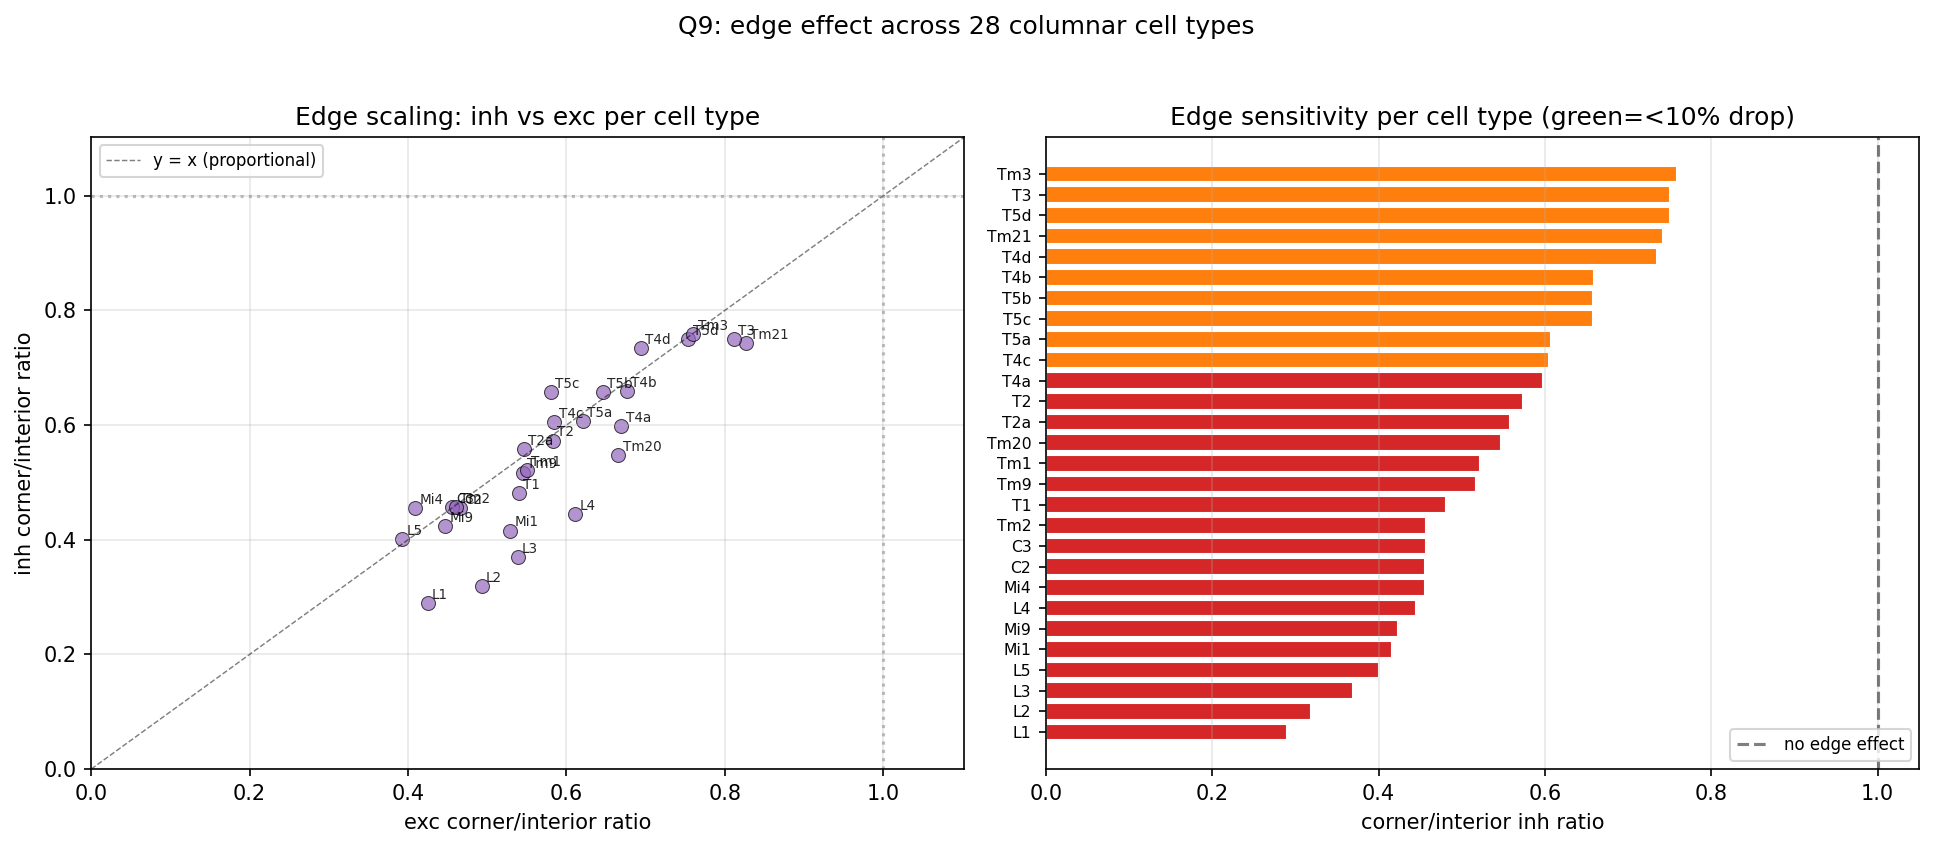
\includegraphics[width=\textwidth]{figures/fig8_multi_type_edge.png}
\caption{29 種の columnar receiver cell type で corner/interior 比 (inh, exc) を集計。左: inh ratio vs exc ratio (y=x diagonal は proportional scaling)。右: corner/interior inh ratio を sorted bar (緑 = 端効果 $<$ 10\%、橙 = 10-40\%、赤 = $>$ 40\%)。}
\label{fig:multi_edge}
\end{figure}

\begin{itemize}
\item 全 29 type で Spearman $\rho$ (n\_neighbors vs inh) は正で有意 → \textbf{端効果は普遍的}
\item corner/interior inh ratio は cell type で大きく異なる:
  \begin{itemize}
  \item Lamina monopolar (L1--L5): 0.29--0.40 (端で最も大きく落ちる)
  \item Mi / Tm 系: 0.42--0.55
  \item T4 / T5 系: 0.60--0.75 (端でも 60--75\% 残る)
  \item Tm3, T3, Tm21: 0.74--0.76 (端効果ほぼ無し)
  \item Tm4: 0.60 (中間的)
  \end{itemize}
\item inh\_frac\_delta (corner $-$ interior): 大半で $|\Delta| < 0.05$ → \textbf{E/I balance は全 type で preserved}
\item 例外: L1 だけ $-0.116$ と特異的に大きく、端では相対的に excitatory 寄り
\end{itemize}

\textbf{compensation 型の cell type は無し}。projection neuron (T4/T5) は端効果が相対的に弱い (入力柱の範囲が広く近傍数の絶対的影響が薄まるためと推定される)。

\section{拡張解析: 構造から計算へ}\label{sec:extended}

Q1--Q9 は側抑制が「量的に広く、wide-field に空間を覆う」という\emph{構造}を量化した。本節では一段進み、その配線が実際にどのような\emph{計算}を実装しているかを連結体から推定する (解析の詳細は \texttt{notebook/lateral\_inhibition\_extended.ipynb}、図は \texttt{generate\_figures.py})。

\subsection{Q10: T4/T5 の方向選択性と入力の空間オフセット}\label{sec:q10}

ON (T4) / OFF (T5) 運動検出器は各個眼柱に 4 亜型 (a/b/c/d) を持ち、それぞれ 4 基本方位の運動に選択的である \cite{maisak2013}。古典的モデルでは方向選択性は\textbf{興奮と抑制 (あるいは速い/遅い入力) の空間オフセット}から生じる。T4 では中心興奮 (Mi1/Tm3) に対し、抑制源 \textbf{Mi9} (GluCl 経由で抑制性) と \textbf{Mi4} (GABA) が home column の反対側に配置されると予測される。

各 cell について columnar 入力の \texttt{syn\_count} 重み付き重心を home 基準の $(\Delta p, \Delta q)$ で求め、per-cell の dipole ベクトル (T4: $\mathrm{Mi9}-\mathrm{Mi4}$、T5: $\mathrm{Tm9}-\mathrm{Tm2}$) の角度を取り、亜型ごとに円形平均・resultant $R$・Rayleigh 検定を計算した (図 \ref{fig:t4t5})。

\begin{figure}[htb]
\centering
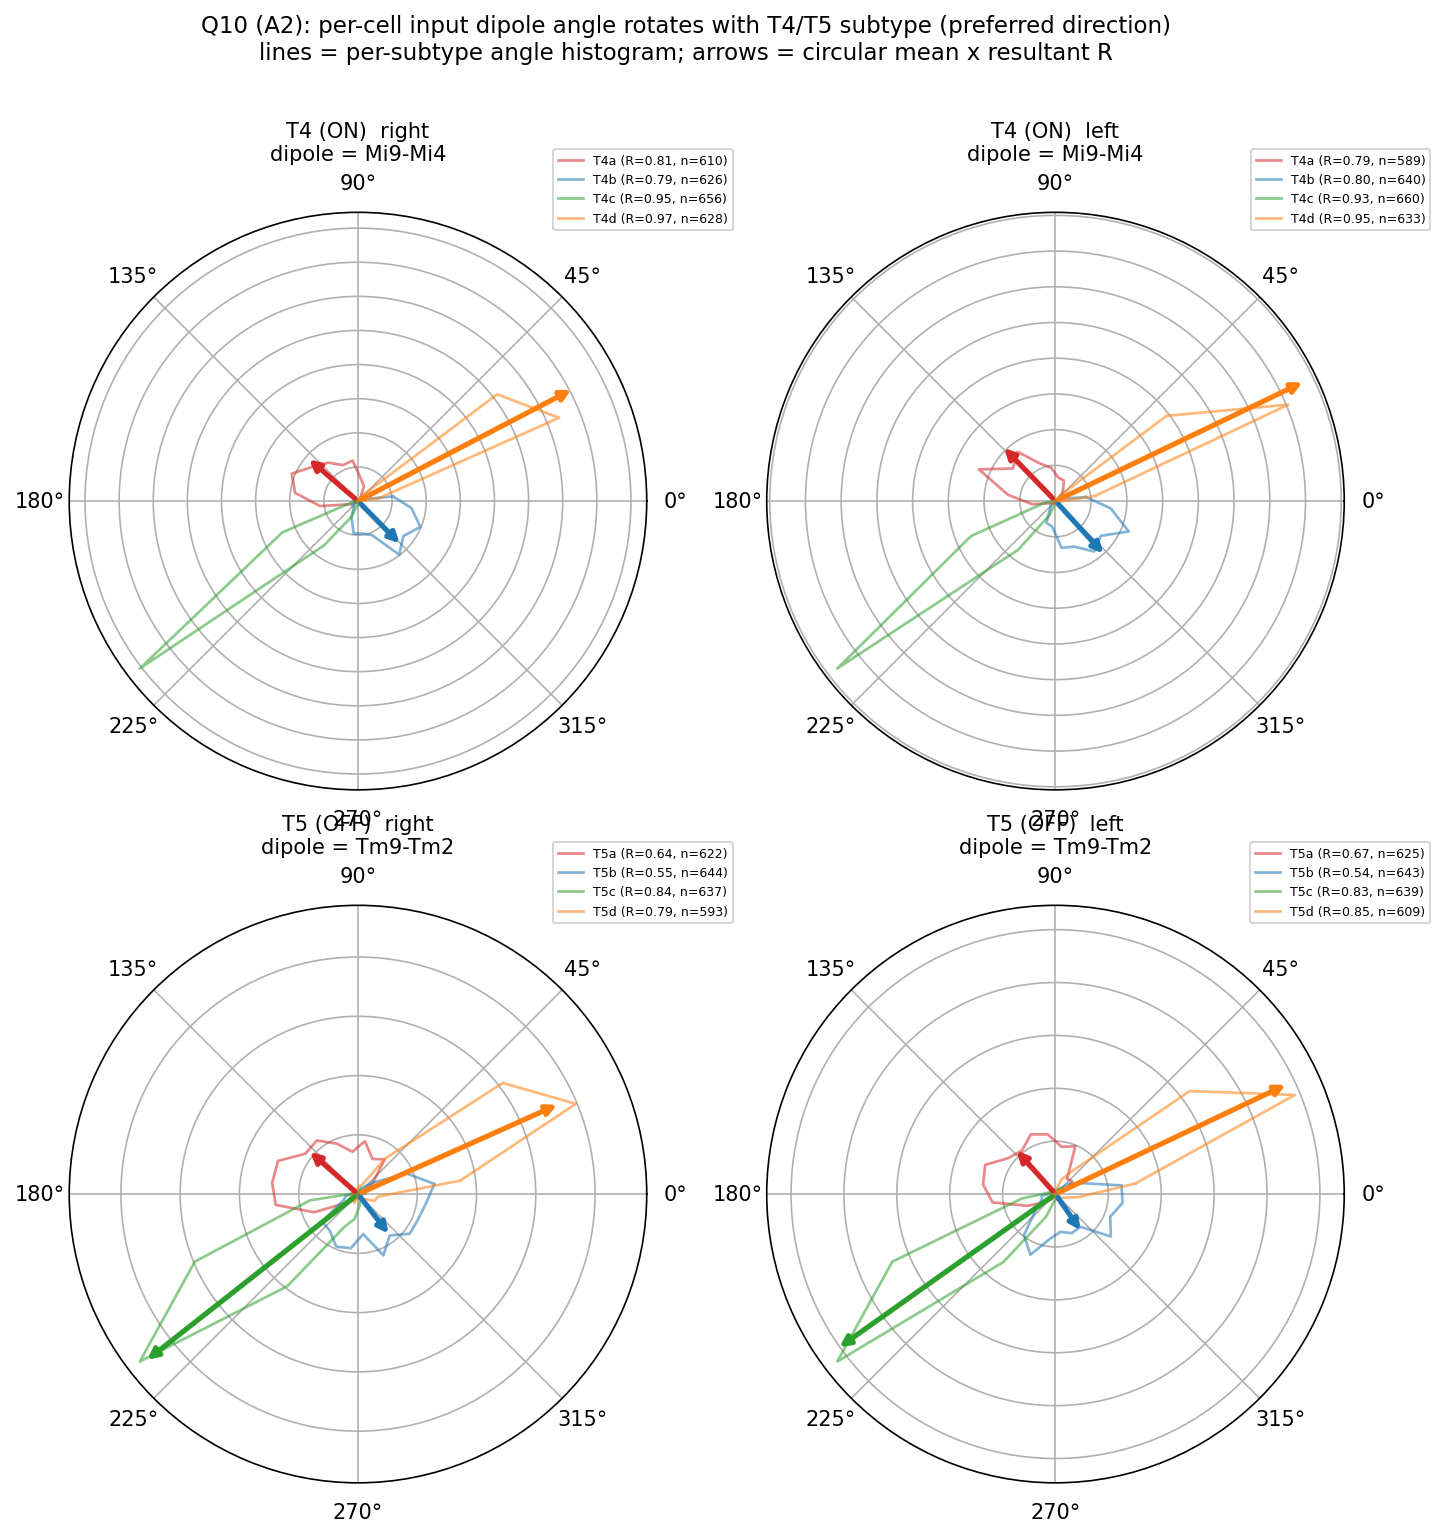
\includegraphics[width=0.72\textwidth]{figures/fig10_t4t5_offset.png}
\caption{T4 (ON) / T5 (OFF) の per-cell 入力 dipole 角の分布 (極座標、pathway $\times$ 半球)。各色が亜型、線はその亜型の角度ヒストグラム、矢印は円形平均を resultant $R$ で重み付けたもの。dipole 軸が亜型で回転し、対向ペア (a/b, c/d) は反平行、水平ペアと垂直ペアの軸はほぼ直交する。}
\label{fig:t4t5}
\end{figure}

結果は明快である:
\begin{itemize}
\item 全 8 亜型 $\times$ 両半球で dipole 角は強く集中する (Rayleigh $p \approx 10^{-80}$ -- $10^{-256}$)
\item 対向ペアは反平行 (T4a/b $\Delta \approx 175^\circ$, T4c/d $\approx 170^\circ$)、水平ペアと垂直ペアの軸はほぼ直交 ($\Delta \approx 78$--$84^\circ$; 完全な $90^\circ$ でないのは hex 格子上の 4 方位が直交しないため、むしろ妥当)
\item \textbf{両半球で角度が数度内で一致}し、さらに \textbf{T4 と T5 で同字亜型の軸が一致} する (例: T4a $139.5^\circ \approx$ T5a $138.7^\circ$; 同方位選択性同士の内部整合)
\end{itemize}
連結体だけから、方向選択性の\textbf{空間オフセット仮説}が全脳スケール・複数内部対照付きで支持される。これは少数カラムの EM 研究 \cite{takemura2017, shinomiya2019} を全脳・全細胞の定量検定へ拡張したものと位置づけられる。絶対方位 (背腹/前後軸) と既知の preferred direction の整合は、hex 軸を視空間軸へ写す surface fitting を要する今後の課題である。

\subsection{Q11: center--surround 受容野 (Mexican-hat)}\label{sec:q11}

側抑制の本質は\textbf{center--surround 拮抗}である。各 columnar 標的 $T$ が受ける入力を home からの hex 距離 $\Delta$ の関数として再構成した: 興奮 $E(\Delta)$ は直接 columnar 興奮入力の分布、抑制 $I(\Delta)$ は\textbf{二シナプス性 surround} — 抑制 partner $J$ が自身の入力を pool する column 群を $T$ の home 基準で集計したもの (= 抑制が「見ている」視空間) である。視覚葉の抑制源の多くは座標を持たない wide-field 介在 (Pm/Dm/CT1) なので、surround は $J$ の入力 footprint を経た二シナプス性再構成で初めて現れる (図 \ref{fig:censurr})。

\begin{figure}[htb]
\centering
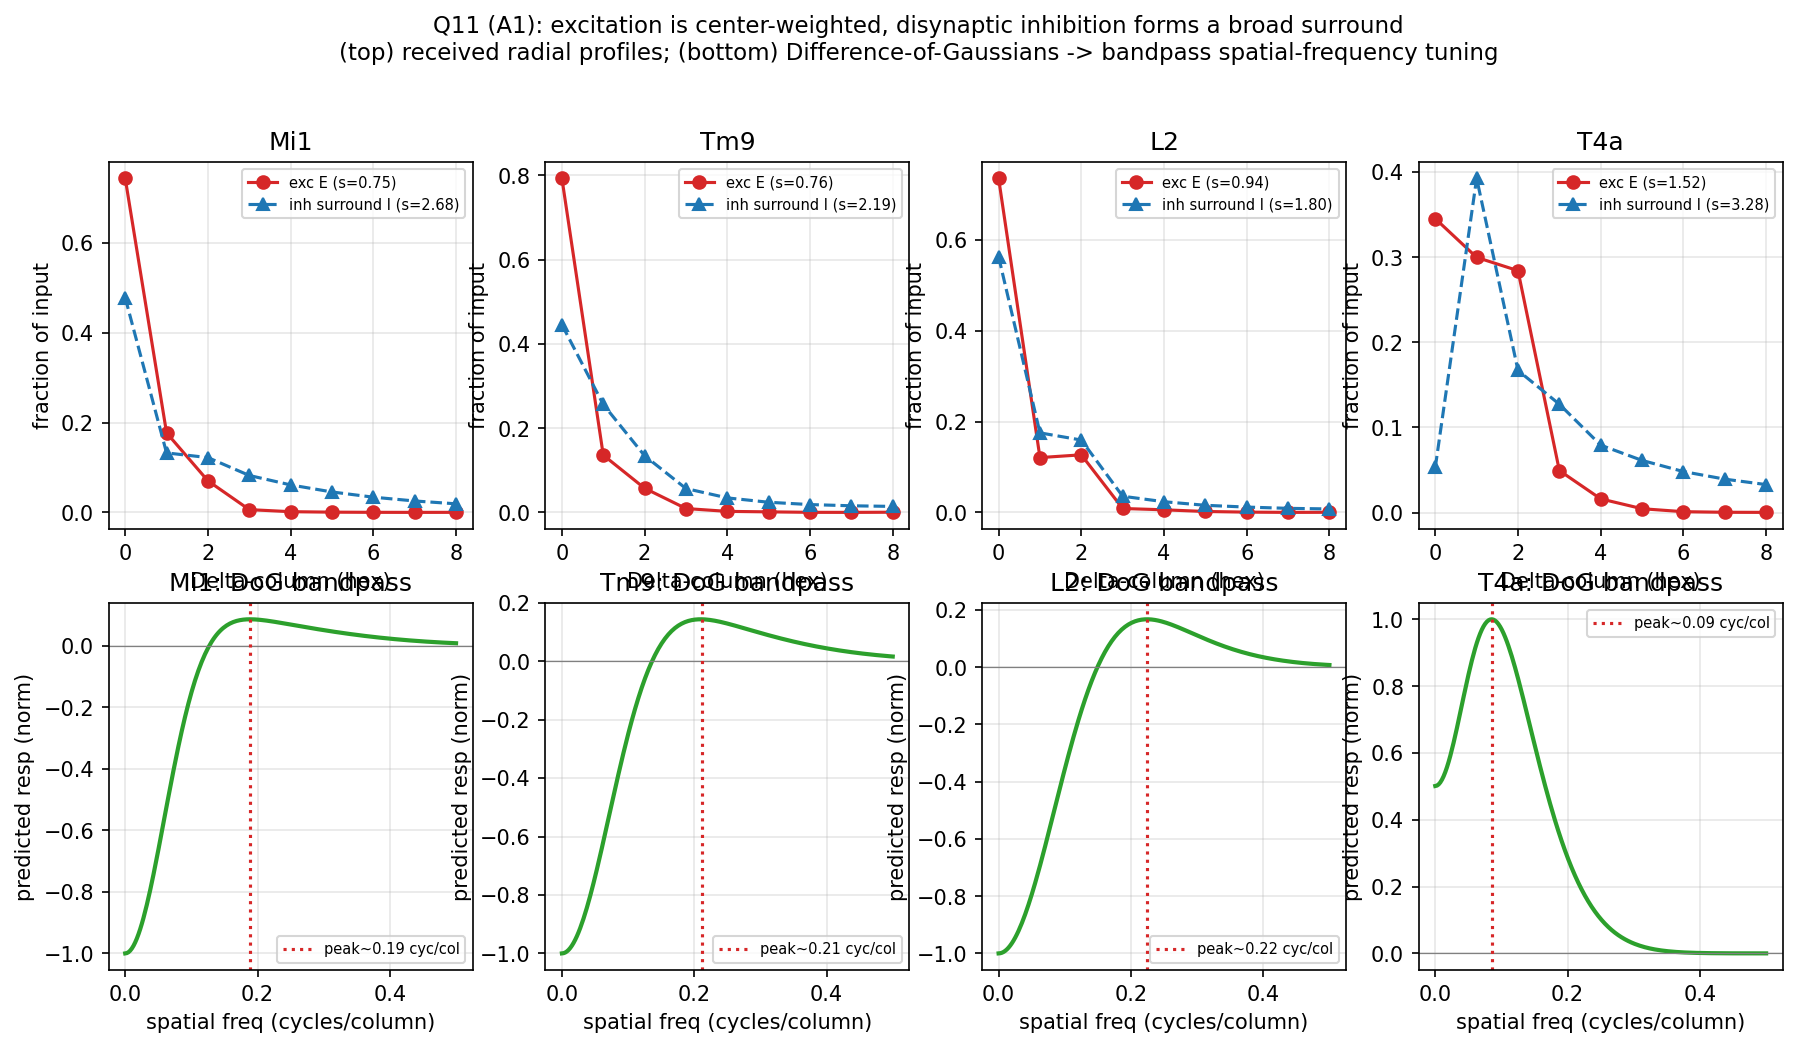
\includegraphics[width=\textwidth]{figures/fig11_center_surround.png}
\caption{(上段) 各標的が受ける興奮 $E(\Delta)$ (赤) と二シナプス性抑制 surround $I(\Delta)$ (青) の radial profile。(下段) これらを Difference-of-Gaussians とみなしたときの予測空間周波数応答。Mi1/Tm9/L2 は中心興奮・周辺抑制でバンドパス ($\sim$0.2 cycles/column にピーク) を示す。}
\label{fig:censurr}
\end{figure}

興奮は鋭く中心集中 (RMS 半径 $\sim$0.3--0.8 柱、home に 7--8 割) する一方、二シナプス性抑制 surround は明確に広く ($\sim$1--2 柱)、surround/center 半径比は中央値 2.5 であった。Mi1/Tm9/L2 のような columnar 中継細胞は DoG とみなすと\textbf{バンドパス} (一様照明を抑えコントラスト・エッジを強調) の空間周波数特性を予測でき、これは Q4 の「抑制 cell の\emph{出力}が広い」を、標的が\emph{受ける}空間演算として裏返したものである。一方 T4a (運動検出器) は中心集中せず DoG ピークも低い — 空間コントラストではなく方向 (Q10) を計算する細胞であることと整合する。なお単シナプス抑制だけでは home 集中に見え (例: L1 から Mi1 への home-column 入力)、surround は二シナプス性再構成でのみ現れる点が重要である。

\subsection{Q12: 抑制マイクロ回路モチーフの census}\label{sec:q12}

量・空間に続き、抑制の\textbf{トポロジー}を分類した。各 cell type を出力 sign で inh/exc dominant に分類し、(a) \emph{脱抑制}: 抑制シナプスが抑制性細胞を標的にする割合、(b) \emph{相互抑制}: $A\to B$ と $B\to A$ が両方抑制な type ペア、(c) \emph{feedforward 抑制 (FFI)}: 共通の興奮駆動が標的とその抑制源を同時に駆動する motif \cite{mauss2015}、を定量した (図 \ref{fig:motif})。

\begin{figure}[htb]
\centering
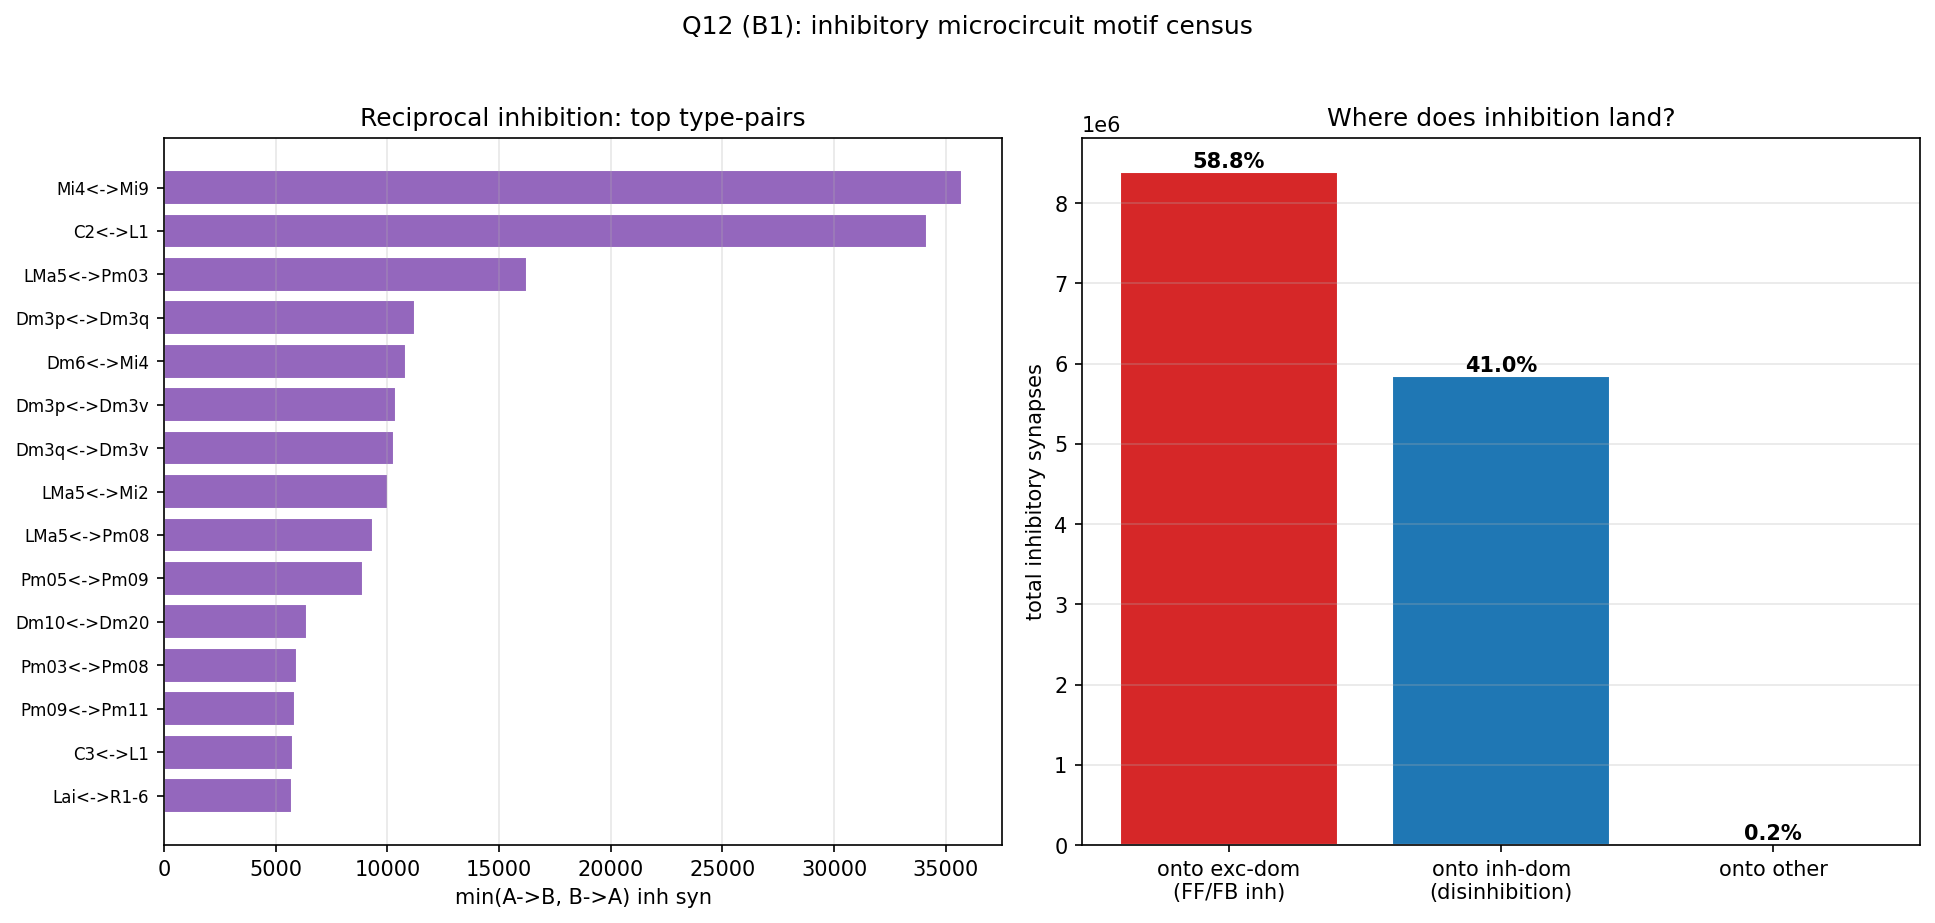
\includegraphics[width=\textwidth]{figures/fig12_motif_census.png}
\caption{(左) 相互抑制を持つ type ペアの上位 (両方向 $\geq 500$ inh syn)。(右) 全抑制シナプスの着地先を post 細胞の出力 sign で分類した内訳。約 41\% が抑制性細胞 (脱抑制) を標的とする。}
\label{fig:motif}
\end{figure}

\begin{itemize}
\item \textbf{全抑制シナプスの 41\% が抑制性細胞を標的} (脱抑制基盤) — Q1 の「44\% が抑制」は「うち約 4 割は抑制を抑制している」と再解釈できる
\item 相互抑制は 326 type-pair に及び、筆頭が運動回路の \textbf{Mi4$\leftrightarrow$Mi9}、ほか Dm3p/q/v の三つ巴、Pm 系 (Pm03/05/08/09) の網
\item FFI では \textbf{Mi1 が T4a を駆動しつつ T4a の抑制源 Mi9/Mi4 をも駆動} する (運動回路の feedforward 抑制) ことが定量化される
\end{itemize}
ただし C2/C3/L1 や Lai/R1-6 等の一部ペアは L1 が ML で抑制ラベルとされる点に由来する見かけであり、確率的 nt 推定値 (\texttt{gaba\_avg} 等) でのロバスト性確認が望ましい。

\subsection{Q13: M 層 (深さ) 解像の抑制アトラス}\label{sec:q13}

medulla は M1--M10 の層構造を持ち、層ごとに異なる計算が走る。\texttt{synapse\_coordinates.csv} の 3D 座標から、右半球 Mi1 の synapse 重心群を PCA した最小分散軸を局所深さ法線とし、Mi1 の深さ分布を medulla 厚 $[0, 1]$ に較正した (Mi1 = 深さ定規; 図 \ref{fig:mlayer})。

\begin{figure}[htb]
\centering
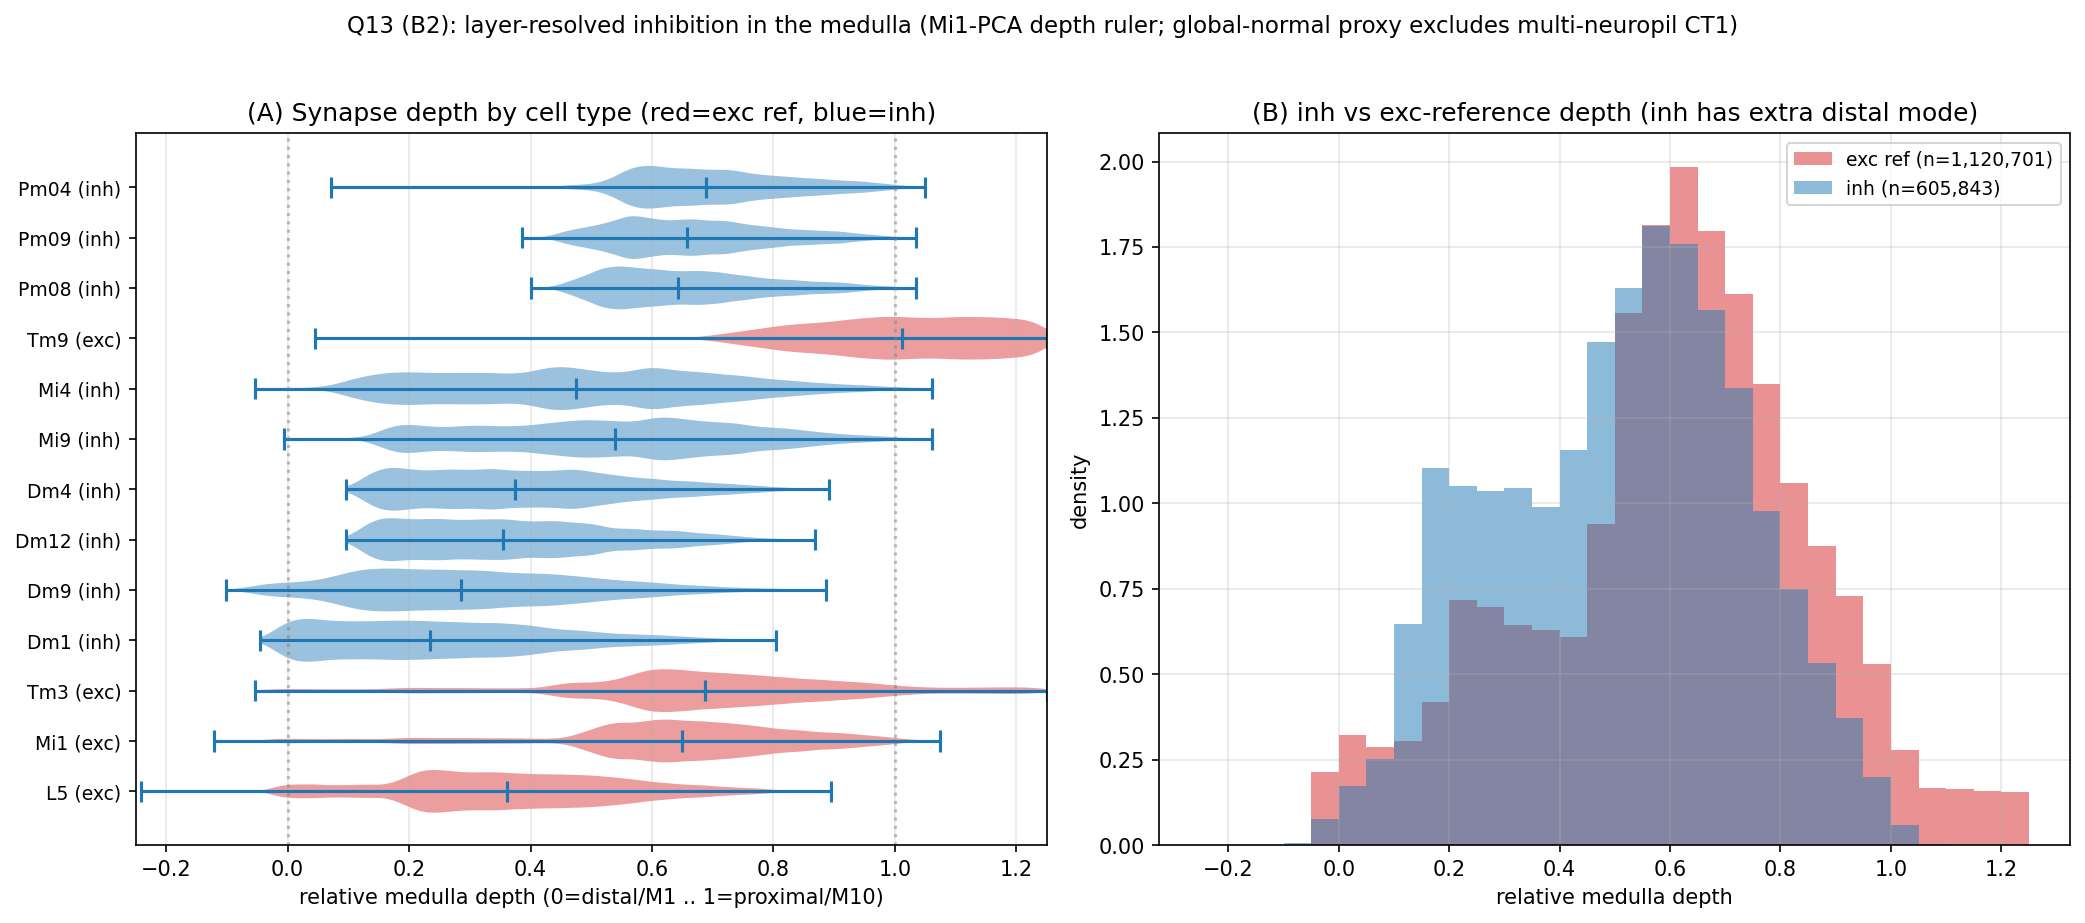
\includegraphics[width=\textwidth]{figures/fig13_mlayer_atlas.png}
\caption{(A) cell type 別の synapse 深さ分布 (赤 = 興奮 reference、青 = 抑制)。(B) 抑制 vs 興奮 reference の深さヒストグラム。Dm は遠位、Pm は近位、Mi4/Mi9 は中層に分離し、抑制は遠位に追加モードを持つ。}
\label{fig:mlayer}
\end{figure}

\textbf{Dm 系は遠位 (median 深さ 0.24--0.37)・Pm 系は近位 (0.64--0.69)} に教科書通り分離し、Mi4/Mi9 は中層 (0.48--0.54) に位置する。抑制シナプス全体は興奮 reference に比べ\textbf{遠位に追加モード}を持つ。層ごとに抑制の担い手と量が異なることが connectome から復元できる。単一 global 法線は medulla の曲率を無視する近似であり、全 medulla を 1 cell で覆う CT1 はこの proxy では深さが破綻するため除外した (柱ごとの surface fitting による曲率補正が上位版)。

\section{議論}\label{sec:discussion}

\subsection{連結体レベルで支持される側抑制の量的特徴}

Q1--Q5, Q8 を通じて、以下の四点が連結体データで強く支持された:
\begin{enumerate}
\item \textbf{量的な広さ}: 全シナプスの約半分 (44\%) が抑制性
\item \textbf{多数の専用 inhibitory interneuron 群}: inh-dominant cell type が 205 種以上存在
\item \textbf{matched 比較で wide-field 構造}: Pm/Dm/Sm の中核 family が columnar excitatory cell の約 3.35--5.73 倍の column 範囲をカバー
\item \textbf{古典回路の再現}: Lai, Dm/Pm 系, Dm8 など全て連結体で形態的に確認
\end{enumerate}

\subsection{Q7--Q9: 境界処理は補償されない}

意外にも、端 column の cell では \textbf{特定の補償機構 (例: CT1 のような global source の比重増加) は存在しなかった}。全ての inh source が proportional に減り、E/I balance のみ保たれる構造である。これは以下のように解釈できる:

\begin{itemize}
\item 端 column の出力強度は中央より弱いが、E/I 比が保たれるため発火パターンは大きく崩れない
\item 視覚処理が relative comparisons (例: 物体の対比、運動の方向) を中心とする場合、絶対応答強度の低下は致命的ではない可能性
\item 補償があるとすれば、後段の \textbf{ゲイン制御 (gain control)} や \textbf{活動依存的なホメオスタシス (homeostatic plasticity)} で行われており、連結体上には現れない
\item 行動レベルでは、注視や運動補正で「端で見えにくい部分」を中心視に持ってくる戦略が取られる可能性
\end{itemize}

\subsection{Q4 metric の限界と input-side で測る Dm8}

Q4 の Δcolumn metric は post が columnar (column\_assignment 入り) であることを前提にする。よって出力が wide-field 細胞ばかりに向かう Dm8 のような color circuit cell には適用できない。代替手段として Q6 で示した「input 側 column footprint」が有効で、教科書記述の Dm8 receptive field がきれいに再現された。

複数のターゲットが column\_assignment 外の cell type (Sm, Tm5*, Dm9 等) は、Q4 metric では `NaN` になるが Q6 と同じ input-side アプローチで個別に評価可能である。

\subsection{ML nt\_type 予測の限界}

FlyWire の \texttt{nt\_type} はシナプス画像からの機械学習推定値で、cell type 単位では大きく信頼できるものの、個別細胞では誤り得る。本解析で最も顕著な例は Dm9 で、文献では GABA 性とされるが ML 予測では出力 syn の 97\% が ACH であった。形態的には他の Dm と同様の wide-field 構造を持つので、ラベル / 予測の問題と思われる。特定 cell type の機能を主張するときは、ML 予測ではなく文献やトランスクリプトーム実測値を優先することが望ましい。

\subsection{構造から計算へ (Q10--Q13 の含意)}

Q10--Q13 は、側抑制の配線が具体的な\emph{計算}を実装していることを示す。\textbf{(i) 方向選択性}: T4/T5 の抑制入力の空間 dipole が亜型で回転し、両半球・ON/OFF 経路で整合する (\S\ref{sec:q10})。\textbf{(ii) 空間バンドパス}: columnar 中継細胞は中心興奮・周辺抑制の Mexican-hat を持ち、一様照明を抑えてエッジ・コントラストを強調するフィルタとして働く (\S\ref{sec:q11})。\textbf{(iii) 脱抑制}: 抑制の約 4 割が抑制性細胞を標的とし、単純な「抑える」配線ではなく多段の制御構造を成す (\S\ref{sec:q12})。\textbf{(iv) 層分業}: 抑制は M 層ごとに担い手が異なる (\S\ref{sec:q13})。これらは Q1--Q9 が示した「量的に広い wide-field 抑制」という基盤の上に、\emph{何が計算されているか}を与える。いずれも connectome 構造からの推定であり、機能の確定には activity / behavior データが要る点は引き続き限界である。

\section{限界と注意点}\label{sec:limitations}

\begin{itemize}
\item \texttt{nt\_type} の多くは ML 予測で、信頼度フィルタを入れていない。$\text{nt\_type\_score} < 0.5$ を除外すると数値はやや変わる
\item GLUT を一律抑制扱いした。Drosophila でも GLUT 興奮性シナプスは存在する
\item Q4 の column-based metric は post が同半球 columnar target である edges のみで計算しており、全 optic-lobe synapse の 35.2\% を直接観測する部分 metric である。Dm/Pm/Sm 同士のように wide-field 細胞間 connection は除外される (Dm8 で見たように一部 cell type ではこれが過小評価バイアスとなる)
\item Mi1 proxy による column 投影は medulla 内では妥当性が高い (Spearman $\rho \approx 0.94$) が、深い M-layer の synapse では小さな column 同定誤差が混入する可能性がある
\item M-layer (M1--M10) 単位の stratification 解析は本報告ではしていない。"lateral within the same M-layer" の strict 検証には z-coord ベースの M-layer 推定が必要
\item Q7 / Q9 の境界効果は接続強度 (syn count) で測ったが、機能側の補償 (gain control 等) は connectome には現れない
\item 「side inhibition の機能的検証」には activity / behavioral データが必要
\end{itemize}

\section{まとめ}

FlyWire 連結体データを 9 つの問いに分解して解析した結果、ショウジョウバエ視覚系における側抑制は (1) 全シナプスの 44\% を占める量的広さ、(2) 200 種以上の inhibitory interneuron 群、(3) Pm/Dm/Sm を中心とした wide-field 構造 (抑制 dominant cell type は興奮 dominant の約 3.35 倍の lateral spread)、(4) Lai / Dm8 等の古典回路の再現 という四点で連結体レベルで強く支持されることが分かった。境界処理については特定の補償機構は無く、E/I balance を保ちつつ proportional に scale down するという構造で、補償があるとすれば後段のゲイン制御や行動レベルで行われている可能性が高い。Dm8 のように output が wide-field 細胞ばかりの cell は Q4 metric では測れないが、input 側 (R7 column footprint) を集計することで教科書記述の receptive field が確認できる。さらに拡張解析 (Q10--Q13) は、この抑制配線が T4/T5 の方向選択性 (入力の空間オフセット)、columnar 細胞の center--surround 受容野 (空間バンドパス)、約 41\% に及ぶ脱抑制、M 層ごとの役割分担という\textbf{具体的な計算}を実装していることを連結体から示した。

\bigskip
\noindent\textbf{ソースコードと再現性.} 本解析の全ソースコード (ノートブック + LaTeX + 図生成スクリプト) は \texttt{flywire\_analysis} リポジトリで公開されている。ノートブックは \texttt{notebook/lateral\_inhibition.ipynb} に Q1--Q9 を順に格納してあり、図 1--8 は \texttt{report/lateral\_inhibition/generate\_figures.py} で再生成可能。

\begin{thebibliography}{9}

\bibitem{flywire2024}
S. Dorkenwald, A. Matsliah, A. R. Sterling, et al.\\
\textit{Neuronal wiring diagram of an adult brain.}
Nature 634, 124--138 (2024).

\bibitem{gao2008}
S. Gao, S.-Y. Takemura, C.-Y. Ting, et al.\\
\textit{The neural substrate of spectral preference in Drosophila.}
Neuron 60, 328--342 (2008).

\bibitem{karuppudurai2014}
T. Karuppudurai, T.-Y. Lin, C.-Y. Ting, et al.\\
\textit{A hard-wired glutamatergic circuit pools and relays UV signals to mediate spectral preference in Drosophila.}
Neuron 81, 603--615 (2014).

\bibitem{maisak2013}
M. S. Maisak, J. Haag, G. Ammer, et al.\\
\textit{A directional tuning map of Drosophila elementary motion detectors.}
Nature 500, 212--216 (2013).

\bibitem{takemura2017}
S. Takemura, A. Nern, D. B. Chklovskii, et al.\\
\textit{The comprehensive connectome of a neural substrate for `ON' motion detection in Drosophila.}
eLife 6, e24394 (2017).

\bibitem{shinomiya2019}
K. Shinomiya, G. Huang, Z. Lu, et al.\\
\textit{Comparisons between the ON- and OFF-edge motion pathways in the Drosophila brain.}
eLife 8, e40025 (2019).

\bibitem{mauss2015}
A. S. Mauss, M. Meier, E. Serbe, A. Borst.\\
\textit{Optogenetic and pharmacologic dissection of feedforward inhibition in Drosophila motion vision.}
J. Neurosci. 34, 2254--2263 (2014).

\bibitem{column_validation}
本リポジトリの \texttt{notebook/column\_assignment\_validation.ipynb} 参照。
Spearman $\rho \approx 0.94$ (Mi1 right-hemi で hex distance と物理 centroid 距離の相関)。

\end{thebibliography}

\end{document}
